%%%%%%%%%%%%%%%%%%%%%%%%%%%%%%%%%%%%%%%%%%%%%%%%%%%%%%%%%%%%%%%%
%%                                                            %%
%%   essentialsOfLatin, Italian translation 2017              %%
%%                                                            %%
%% From:  Henry C. Pearson, Essentials Of Latin For Beginners %%
%%        (1915, New York, American Book Company)             %%
%%                                                            %%
%%    https://archive.org/details/essentialslatin04peargoog   %%
%%                                                            %%
%% Translated by g.p.ciceri <gp.ciceri@gmail.com>             %%
%% ---------------------------------------------------------- %%
%% This translation is Licensed under                         %%
%% Creative Commons Attribution-ShareAlike 4.0 International  %%
%% https://creativecommons.org/licenses/by-sa/4.0/            %%
%%                                                            %%
%%%%%%%%%%%%%%%%%%%%%%%%%%%%%%%%%%%%%%%%%%%%%%%%%%%%%%%%%%%%%%%%

% āēīōū
% ăĕĭŏŭ




\documentclass[nols]{tufte-handout}

%\geometry{showframe} % display margins for debugging page layout

\usepackage{fontspec}
\usepackage{ifxetex}
\setmainfont[Path=./fonts/palatino-linotype/, ItalicFont=palai.ttf, BoldFont=palab.ttf]{pala.ttf}


% \defaultfontfeatures{Mapping=tex-text}
% \setromanfont[Path=./fonts/TeX-Gyre-Schola/,Mapping=tex-text]{TeX Gyre Schola}
% \setsansfont[Path=./fonts/TeX-Gyre-Heros/,Scale=MatchLowercase,Mapping=tex-text]{TeX Gyre Heros}
% \setmonofont[Path=./fonts/TeX-Gyre-Cursor/,Scale=MatchLowercase]{TeX Gyre Cursor}

\usepackage{lipsum}
\usepackage{url}
\usepackage{longtable}
\usepackage{stackengine}

\usepackage{graphicx} % allow embedded images
  \setkeys{Gin}{width=\linewidth,totalheight=\textheight,keepaspectratio}
  \graphicspath{{graphics/}} % set of paths to search for images
\usepackage{amsmath}  % extended mathematics
\usepackage{booktabs} % book-quality tables
\usepackage{units}    % non-stacked fractions and better unit spacing
\usepackage{multicol} % multiple column layout facilities
\usepackage{lipsum}   % filler text
\usepackage{fancyvrb} % extended verbatim environments
  \fvset{fontsize=\normalsize}% default font size for fancy-verbatim environments

% Standardize command font styles and environments
\newcommand{\doccmd}[1]{\texttt{\textbackslash#1}}% command name -- adds backslash automatically
\newcommand{\docopt}[1]{\ensuremath{\langle}\textrm{\textit{#1}}\ensuremath{\rangle}}% optional command argument
\newcommand{\docarg}[1]{\textrm{\textit{#1}}}% (required) command argument
\newcommand{\docenv}[1]{\textsf{#1}}% environment name
\newcommand{\docpkg}[1]{\texttt{#1}}% package name
\newcommand{\doccls}[1]{\texttt{#1}}% document class name
\newcommand{\docclsopt}[1]{\texttt{#1}}% document class option name
\newenvironment{docspec}{\begin{quote}\noindent}{\end{quote}}% command specification environment

% concetti morfosintattici
\usepackage{xspace} 
\newcommand{\noun}{\textsc{sostantivo}\xspace}
\newcommand{\nouns}{\textsc{sostantivi}\xspace}
\newcommand{\adject}{\textsc{aggettivo}\xspace}
\newcommand{\adjects}{\textsc{aggettivi}\xspace}
\newcommand{\gnumber}{\textsc{numero}\xspace}
\newcommand{\gnumbers}{\textsc{numeri}\xspace}
\newcommand{\gender}{\textsc{genere}\xspace}
\newcommand{\genders}{\textsc{generi}\xspace}
\newcommand{\gcase}{\textsc{caso}\xspace}
\newcommand{\gcases}{\textsc{casi}\xspace}
\newcommand{\tense}{\textsc{tempo}\xspace}
\newcommand{\mood}{\textsc{modo}\xspace}
\newcommand{\gverb}{\textsc{verbo}\xspace}
\newcommand{\gverbs}{\textsc{verbi}\xspace}
\newcommand{\adjective}{\textsc{aggettivo}\xspace}
\newcommand{\nom}{\textsc{nom}\xspace}
\newcommand{\gen}{\textsc{gen}\xspace}
\newcommand{\dat}{\textsc{dat}\xspace}
\newcommand{\acc}{\textsc{acc}\xspace}
\newcommand{\voc}{\textsc{voc}\xspace}
\newcommand{\abl}{\textsc{abl}\xspace}
\newcommand{\gexit}{\textsc{uscita}\xspace}
\newcommand{\gexits}{\textsc{uscite}\xspace}
\newcommand{\declinazione}{\textsc{declinazione}\xspace}
\newcommand{\masc}{\textsc{maschile}\xspace}
\newcommand{\femm}{\textsc{femminile}\xspace}
\newcommand{\neut}{\textsc{neutro}\xspace}

\newcommand{\indic}{\textsc{indicativo}\xspace}
\newcommand{\imper}{\textsc{imperativo}\xspace}
\newcommand{\gcong}{\textsc{congiuntivo}\xspace}
\newcommand{\ott}{\textsc{ottativo}\xspace}
\newcommand{\partic}{\textsc{participio}\xspace}
\newcommand{\infin}{\textsc{infinito}\xspace}

\newcommand{\pres}{\textsc{presente}\xspace}
\newcommand{\imperf}{\textsc{imperfetto}\xspace}
\newcommand{\aor}{\textsc{aoristo}\xspace}
\newcommand{\fut}{\textsc{futuro}\xspace}
\newcommand{\perf}{\textsc{perfetto}\xspace}
\newcommand{\pperf}{\textsc{piuccheperfetto}\xspace}

\newcommand{\sing}{\textsc{singolare}\xspace}
\newcommand{\plur}{\textsc{plurale}\xspace}
\newcommand{\dual}{\textsc{duale}\xspace}

\newcommand{\si}{\textsc{sing}\xspace}
\newcommand{\pl}{\textsc{plur}\xspace}
\newcommand{\du}{\textsc{dual}\xspace}

\newcommand{\att}{\textsc{attivo}\xspace}
\newcommand{\med}{\textsc{medio}\xspace}
\newcommand{\pass}{\textsc{passivo}\xspace}
\newcommand{\medpass}{\textsc{medio-passivo}\xspace}


% italianitudini
\renewcommand{\figurename}{Figura}
\renewcommand{\tablename}{Tabella}
\renewcommand{\contentsname}{Indice}

% fix per un qualche problema
\ifxetex
  \newcommand{\textls}[2][5]{%
    \begingroup\addfontfeatures{LetterSpace=#1}#2\endgroup
  }
  \renewcommand{\allcapsspacing}[1]{\textls[15]{#1}}
  \renewcommand{\smallcapsspacing}[1]{\textls[10]{#1}}
  \renewcommand{\allcaps}[1]{\textls[15]{\MakeTextUppercase{#1}}}
  \renewcommand{\smallcaps}[1]{\smallcapsspacing{\scshape\MakeTextLowercase{#1}}}
  \renewcommand{\textsc}[1]{\smallcapsspacing{\textsmallcaps{#1}}}
\fi

% too many float...
\extrafloats{100}
% āēīōū
% ăĕĭŏŭ

\title{Essentials Of Latin. Elementi di Latino. \newline Lezione XI - Prima coniugazione. Parti principali di un verbo. Forma e coniugazione di imperfetto e futuro.}

\author[gpciceri]{a cura di Milagathòs: Milo's help to enjoy humanities.}

\date{24 Febbrajo 2017} % without \date command, current date is supplied


\begin{document}

\hyphenation{co-niu-ga-zio-ne}

\maketitle% this prints the handout title, author, and date

\begin{marginfigure}[-2.5cm]
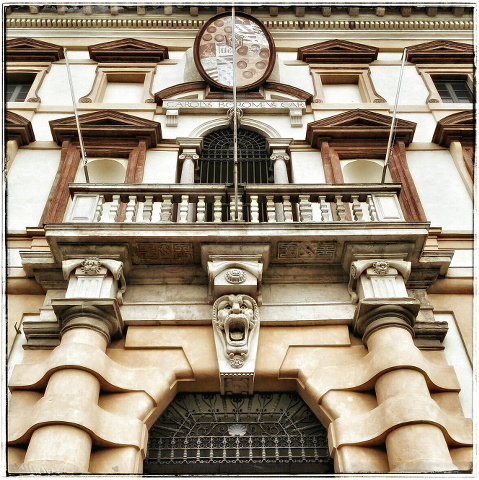
\includegraphics{smallthumb-lesson_I.jpeg}
\setfloatalignment{b}
\end{marginfigure}


\begin{abstract}
\noindent
Queste lezioni riprendono il testo introduttivo al Latino di Pearson\cite{pearson1915}, del quale seguono la numerazione; la struttura di ogni lezione è piuttosto regolare: inizia con \textsc{cenni di morfologia e di sintassi latina}, seguita da un \textsc{piccolo vocabolario} per il lessico; ci sono infine vari \textsc{esercizi} di traduzione e di composizione latina.

\bigskip
\noindent
Lezione XI - Prima coniugazione. Parti principali di un verbo. Forma e coniugazione di imperfetto e futuro.
\end{abstract}

%\printclassoptions

% āēīōū
% ăĕĭŏŭ

\newthought{85.} Ripassa (26.) e (43.). In latino i verbi sono divisi in quattro coniugazioni, 
che si distinguono tra loro per la vocale prima della \textbf{-re} dell'infinito presente attivo. 
Avremo quindi:

\begin{fullwidth}
\begin{table}[!htbp]
  \centering
  \begin{tabular}{r l l}
    %\toprule
	\multicolumn{1}{c}{\textsc{Coniugazione}} & \multicolumn{1}{c}{\textsc{Infinito Presente Attivo}} & \multicolumn{1}{c}{\textsc{Vocale Caratteristica}} \\

    \textsc{I} & \textbf{amāre}, \textit{amare} & \textbf{ā}  \\
    \textsc{II} & \textbf{monēre}, \textit{ammonire} & \textbf{ē}  \\
    \textsc{III} & \textbf{legĕre}, \textit{leggere} & \textbf{ĕ}  \\
    \textsc{IV} & \textbf{audīre}, \textit{ascoltare} & \textbf{ī}  \\
    
    %\bottomrule
  \end{tabular}
  %\caption[bottom]{Prima Declinazione. \textbf{stella, -ae}, f.}
  \label{tab:normaltab}
  %\zsavepos{pos:normaltab}
\end{table}
\end{fullwidth}


\newthought{86. Parti principali del verbo.} Le parti principali, \textit{il paradigma} di un verbo sono (1) l'indicativo presente attivo,
(2) l'indicativo perfetto attivo, (3) il participio perfetto (passivo) singolare neutro, (4) l'infinito presente attivo.
Queste quattro forme verbali devono obbligatoriamente essere apprese, dal momento che da esse si ricavano i temi necessari alla formazione
di ogni singola voce verbale. Questi temi sono: (1) tema del presente, (2) tema del perfetto, (3) tema del participio, e si ricavano in questo modo:

\begin{fullwidth}
\begin{table}[!htbp]
  \centering
  \begin{tabular}{r c c c c}
    %\toprule
	\textsc{Ind.Pres} & \textsc{Ind.Perf} & \textsc{Part.Perf} & \textsc{Inf.Pres} \\

    \textbf{amō}    & \textbf{amāv|ī}   & \textbf{amāt|um}    & \textbf{amā|re}  \\
	\textit{io amo} & \textit{io amai}  & \textit{amato}      & \textit{amare} \\
                    & tema del perfetto & tema del participio & tema del presente \\
 
    %\bottomrule
  \end{tabular}
  %\caption[bottom]{Prima Declinazione. \textbf{stella, -ae}, f.}
  \label{tab:normaltab}
  %\zsavepos{pos:normaltab}
\end{table}
\end{fullwidth}

\newthought{87. Prima Coniugazione, Imperfetto e Futuro.} 

\begin{fullwidth}
\begin{table}[!htbp]
  \centering
  \begin{tabular}{l l l l l}
    %\toprule
	
	\multicolumn{5}{c}{\textsc{Indicativo Imperfetto Attivo}} \\
	
	& \multicolumn{1}{c}{\textsc{Singolare}} & \hspace{20mm} & & \multicolumn{1}{c}{\textsc{Plurale}} \\

    \textsc{1.} & amā\textbf{bam}, \textit{io amavo}   & \hspace{20mm} & \textsc{1.} & amā\textbf{bāmus}, \textit{noi amavamo}    \\
    \textsc{2.} & amā\textbf{bās}, \textit{tu amavi}   & \hspace{20mm} & \textsc{2.} & amā\textbf{bātis}, \textit{voi amavate}    \\
    \textsc{3.} & amā\textbf{bat}, \textit{egli amava} & \hspace{20mm} & \textsc{3.} & amā\textbf{bant}, \textit{essi amavano}    \\
   
	\multicolumn{5}{c}{\textemdash} \\
	
    \multicolumn{5}{c}{\textsc{Indicativo Futuro Attivo}} \\
	
	& \multicolumn{1}{c}{\textsc{Singolare}} & \hspace{20mm} & & \multicolumn{1}{c}{\textsc{Plurale}} \\

    \textsc{1.} & amā\textbf{bō}, \textit{io amerò}   & \hspace{20mm} & \textsc{1.} & amā\textbf{bimus}, \textit{noi ameremo}    \\
    \textsc{2.} & amā\textbf{bis}, \textit{tu amerai}   & \hspace{20mm} & \textsc{2.} & amā\textbf{bitis}, \textit{voi amerete}    \\
    \textsc{3.} & amā\textbf{bit}, \textit{egli amerà} & \hspace{20mm} & \textsc{3.} & amā\textbf{bunt}, \textit{essi ameranno}    \\

    %\bottomrule
  \end{tabular}
  %\caption[bottom]{Prima Coniugazione, Imperfetto.}
  \label{tab:normaltab}
  %\zsavepos{pos:normaltab}
\end{table}
\end{fullwidth}

\newthought{Osservazioni}
\begin{itemize}
\item[\textsc{1.}] La prima persona singolare dell'imperfetto si forma aggiungendo \textbf{-bam} al tema del presente, 
mentre la prima persona singolare del futuro si forma aggiungendo \textbf{-bō} al tema del presente. In questo modo:
	\begin{itemize}
		\item \textbf{amō}	\quad tema del presente \textbf{amā-}	\quad	imperfetto  \textbf{amā-bam}
		\item \textbf{amō}	\quad tema del presente \textbf{amā-}	\quad	futuro  \textbf{amā-bō}
	\end{itemize}
\item[\textsc{2.}] Le terminazioni pesonali (43.) sono le medesime di quelle del presente. 
\end{itemize}

\newthought{88. Esercizio di Coniugazione} Impara le parti principali e coniuga l'indicativo imperfetto e il futuro attivo dei verbi:

\begin{itemize}
\item[\textbf{parō}], \textit{preparare}, \textbf{parō, -as, parāvī, parātum, parāre}
\item[\textbf{laudō}], \textit{lodare, apprezzare}, \textbf{laudō, -as, laudāvī, laudātum, laudāre}
\item[\textbf{culpō}], \textit{incolpare}, \textbf{culpō, -as, culpāvī, culpātum, culpāre}
\item[\textbf{convocō}], \textit{convocare, radunare}, \textbf{convocō, -as, convocāvī, convocātum, convocāre}
\end{itemize}

% āēīōū
% ăĕĭŏŭ

\newthought{89. Vocabolario} 

\begin{multicols}{2}
    \noindent \hangindent=1em \textbf{locus, -ī}, m.; \textbf{locī}, m.pl.;  \textbf{loca}, n.pl.;  \textit{luogo, posto}.  \\
    \noindent \hangindent=1em \textbf{praemium, -ī}, n., \textit{premio, ricompensa}.  \\
    \noindent \hangindent=1em \textbf{pilum, -ī}, n., \textit{giavellotto}.  \\
	\noindent \hangindent=1em \textbf{saxum, -ī}, n., \textit{roccia, pietra, sasso}.  \\
	\noindent \hangindent=1em \textbf{telum, -ī}, n., \textit{arma}.  \\
	\noindent \hangindent=1em \textbf{castra, -ōrum}, n.pl., \textit{accampamento}.  \\
	
	\noindent \hangindent=1em \textbf{idoneus, a, um}, agg., \textit{adatto, idoneo}.  \\
	
	\noindent \hangindent=1em \textbf{parō, -as, -āvī, -ātum, -āre}, v.tr., \textit{preparare}.  \\
	\noindent \hangindent=1em \textbf{comparō, -as, -āvī, -ātum, -āre}, v.tr., \textit{metto assieme, provvedo}.  \\
	
	\noindent \hangindent=1em \textbf{contra}, prep. + \acc, \textit{contro}.  \\
	
	\noindent \hangindent=1em \textbf{hasta, -ae}, f., \textit{lancia}.  \\
	
\end{multicols}
% āēīōū
% ăĕĭŏŭ

\newthought{90. Esercizi di Ripasso}
\\
\textsc{I.} \quad
\textsc{1.}~Galli filiis agricolarum cibum non dant. \quad
\textsc{2.}~Cur fidum nautam culpatis? \quad
\textsc{3.}~Erant in Graecia aedificia pulchra. \quad
\textsc{4.}~In silvam nuntios convocat. \quad
\textsc{5.}~Inopia cibi et vini viros non delectat. \quad
\textsc{6.}~Multi gladii semper in oppido sunt.
\\
\textsc{II.} \quad
\textsc{1.}~O figlio mio, dov'è la mia spada? \quad
\textsc{2.}~Portano il grano nel grande magazzino. \quad
\textsc{3.}~Tu dai molte rose a mia figlia. \quad
\textsc{4.}~Perché l'isola piace ai ragazzi?


\newthought{91. Esercizi}
\\
\textsc{I.} \quad
\textsc{1.}~Culpabat; laudabant; convocabis. \quad
\textsc{2.}~Pugnabimus; comparabas ; dabunt. \quad
\textsc{3.}~Portabimus ; culpabitis ; laudabit. \quad
\textsc{4.}~Bellum contra Gallos parabant. \quad
\textsc{5.}~Praemia idonea viros delectabunt. \quad
\textsc{6.}~Galli in castra cibum et tela portant. \quad
\textsc{7.}~Idoneane praemia comparabitis? \quad
\textsc{8.}~Ubi est locus castris idoneus? \quad
\textsc{9.}~Fili praemium erit pulchrum pilum. \quad
\textsc{10.}~Idoneas hastas viris dabimus. \quad
\textsc{11.}~Multae sagittae et pila sunt in castris. \quad
\textsc{12.}~Galli bellum contra Romands parabunt.
\\
\textsc{II.} \quad
\textsc{1.}~Voi darete; essi davano; ella dava. \quad
\textsc{2.}~noi lodiamo; egli incolperà; noi raduniamo. \quad
\textsc{3.}~Essi porteranno; noi daremo; tu apprezzavi. \quad
\textsc{4.}~Preparavamo un luogo adatto per un accampamento. \quad
\textsc{5.}~Darà una ricompensa a sua figlia. \quad
\textsc{6.}~I Romani preparavano la guerra contro i Galli. \quad
\textsc{7.}~Le armi dei Galli erano sassi e frecce.


\begin{figure}[!b]
  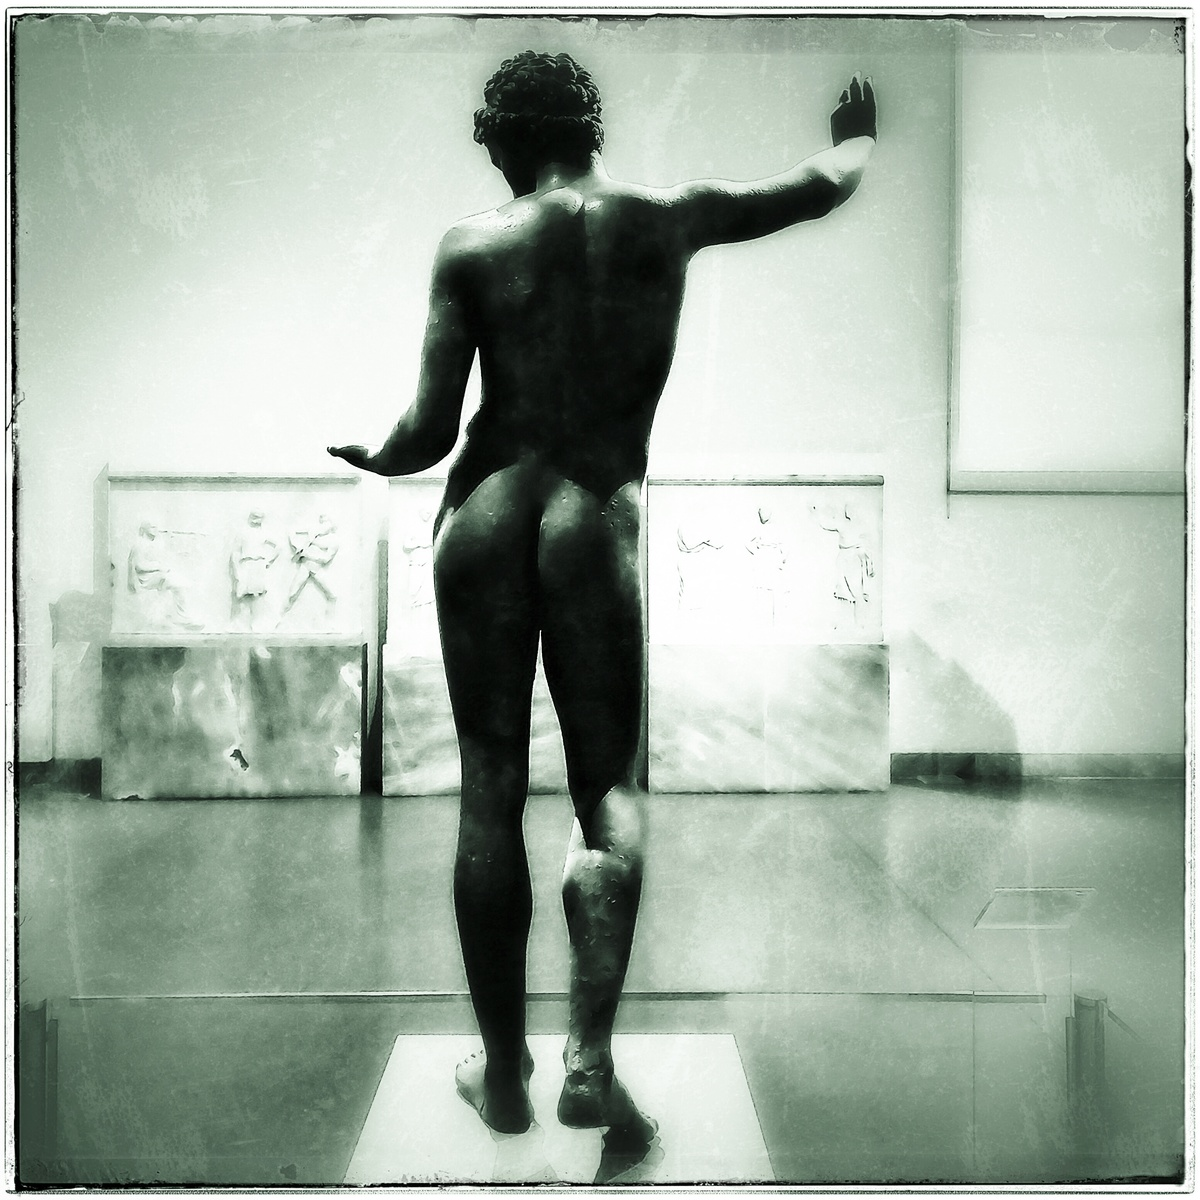
\includegraphics[width=0.8\linewidth]{thumb-lesson_VII.jpeg}
  %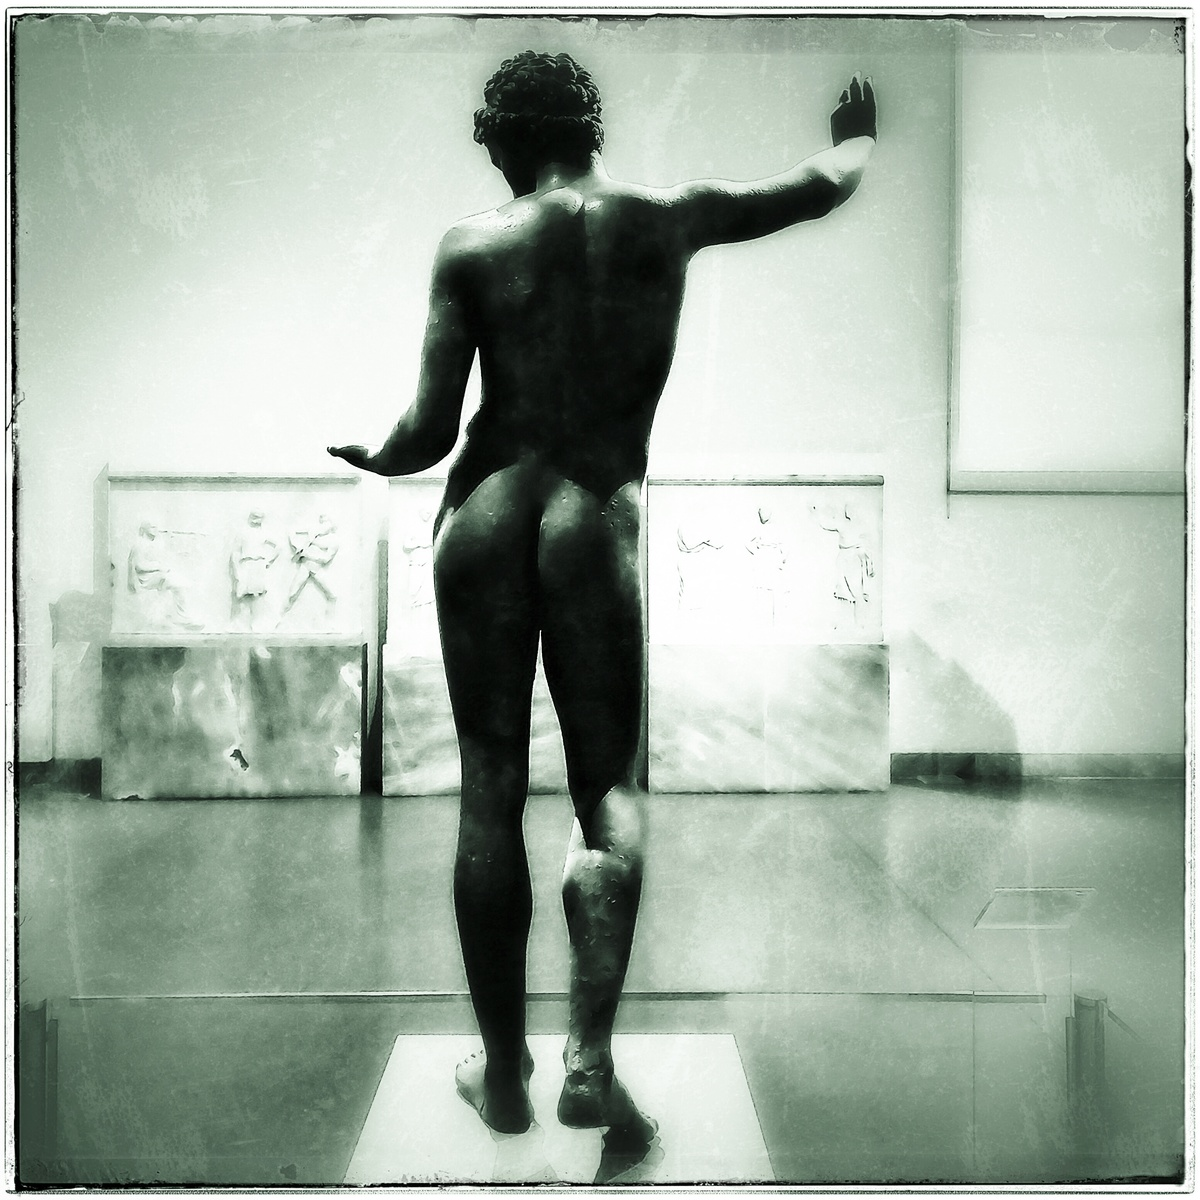
\includegraphics{thumb-lesson_VII.jpeg}
  \caption{Pavia: Almo Collegio Borromeo}
  \label{fig:textfig}
  %\zsavepos{pos:textfig}
  %\setfloatalignment{b}
\end{figure}

 

\nobibliography{latinBiblio}
\bibliographystyle{alpha}


\end{document}
